\documentclass[main.tex]{subfiles}

\begin{document}

\chapter{La dette publique, l'exemple européen}

\textit{Pourquoi les dettes publiques européennes sont elles si élevées, cela constitue-t-il un problème ?}

\begin{definition}[Dette publique]
        L'ensemble des engagements financiers pris sous formes d'emprunts par un État, ses collectivités publiques et ses organismes qui en dépendent directement comme certaines entreprises publiques, les organismes de sécurité sociale, \textit{etc.}
        Tous les pays ont des dettes publiques, même ceux dont les recettes sont supérieures aux dépenses et le patrimoine financier net largement positif. L’État présente donc souvent en fin d’année un solde budgétaire négatif, aussi appelé \emph{déficit public}.
\end{definition}

La dette publique possède certaines caractéristiques qui lui sont propres
\begin{itemize}
        \item La continuité et la perpétuité de l'État. Les prêts à un État sont grâce à cela très surs, même si ce dernier n'est pas solvable immédiatement, il pourra l'être dans le futur. La Révolution française est un bon exemple, la dette fut conservée après l'abolition de la monarchie. Il y a une séparation entre dette d'État et gouvernement
        \item Presque tous les États européens en possèdent une, les États Unis jusqu'au XIX\up{ème} et la Chine jusqu'au XVIII\up{ème} n'en avaient pas, cela était mal perçu
        \item Elle est l'objet d'une méfiance de la part de l'économie politique, elle garde longtemps mauvaise image. Un changement majeur se produit en 1914 avec le début de la Première Guerre mondiale. Keynes met en avant plusieurs atouts du \emph{deficit spending}, on se met à penser que la dette publique est une bonne chose, qu'elle permet aux pays de se développer.
\end{itemize}

\begin{definition}[\textit{Deficit spending}]
        Lorsqu'un gouvernement dépense plus que la somme de ses revenus, selon l'économiste Keynes cela présente deux atouts majeurs
        \begin{enumerate}
                \item Selon lui un niveau de dépense minimal est nécessaire pour maintenir la \emph{demande globale}, c'est à dire la somme des dépenses des particuliers et des entreprises, elle même nécessaire au maintient d'un taux de chômage bas
                \item Le second, et peu être plus important, selon Keynes une dépense d'un dollar de la part du gouvernement peu entrainer une augmentation de la production économique finale d'une valeur de plus d'un dollar. Il s'agit du \emph{multiplier effect}
        \end{enumerate}
\end{definition}

Malgré ce changement dans l'opinion générale, la dette publique reste l'objet de critiques de la part de ses détracteurs. En 1980 par exemple R. Barro et J. Buchanan publient leur critique de cette dernière en la qualifiant de \textit{`plus important problème économique auquel doivent faire face les démocraties occidentales'}.
        
\subsection{Comment l'État emprunte-t-il?}
Les emprunts de l'État français sont très règlementés. On retrouve au 9\up{ème} étage du ministère de l'économie, à Bercy, \emph{l'Agence France Trésor} chargée des emprunts.

\begin{definition}[Agence France Trésor]
        C'est un service à compétence nationale français chargé de gérer la dette et la trésorerie de l'État. Elle a été créée sous le nom d'Agence de la dette par l'arrêté du 8 février 2001, et est rattachée à la Direction générale du Trésor.
\end{definition}

En automne cette dernière émet un projet de loi de finance qui détermine le montant que la France devra emprunter pour l'année suivante. Chaque premier jeudi du mois, la France émet des OAT, \emph{Obligations Assimilables du Trésor Français}, le troisième jeudi du mois elle émet les BTAN, \emph{Bon du trésor à intérêts annuels}.

\begin{definition}[OAT]
        Ce sont des valeurs assimilables du Trésor à moyen et long terme, de maturité de 2 à 50 ans. Les OAT constituent la forme unique du financement à moyen et long terme de l'État, après en avoir été la forme privilégiée sur le seul long terme entre 1985 et 2012. En 2013 les nouveaux titres de référence créés sur le moyen terme, précédemment émis sous la forme de BTAN, sont désormais émis sous la forme d’OAT, comme pour les titres de long terme.
\end{definition}

\begin{definition}[BTAN]
        Ce sont des titres de 2 à 5 ans, aujourd'hui, le dernier \emph{Bon du Trésor à intérêts Annuels} est arrivé à maturité, plus précisément le 25 juillet 2017. L’État a remboursé cette ligne obligataire pour un montant nominal de 19,3 milliards d’euros. À ce jour, il n’y a plus de BTAN s’échangeant sur le marché secondaire. Leur disparition fait partie d'une politique d'uniformisation de la dette de l'État.
\end{definition}

L'AFT travaille avec une vingtaine de banques \emph{Spécialistes Valeurs du Trésor}, qui achètent des titres d'emprunt et fournissent leurs conseils. On retrouve parmi les 18 banques internationales accréditées,
\begin{itemize}
        \item 5 banques américaines dont \emph{Citigroup}, \emph{Bank of America}, \textit{etc.}
        \item 4 banques françaises \emph{BNP Natices, la Société Générale} et \emph{CA}
        \item 1 Suisse, \emph{UBS} 
\end{itemize}

\begin{definition}[Spécialiste Valeurs du Trésor]
        Aussi \emph{primary dealer} en anglais, il s'agit d'une institution financière, banque ou maison de courtage, habilitée à commercer directement avec un gouvernement, l'AFT en France ou la Réserve fédérale aux États Unis.
\end{definition}

        On cherche des pays à forte épargne. En plus de ces banques, les responsables de l'AFT se rendent une à deux fois par mois dans les pays riches comme les États Unis, la Chine, le Japon et la Suisse pour négocier certains emprunts.
        Il ne s'agit en aucun cas de placements de spéculation. Les acheteurs sont les \emph{primary dealers}, puis sur le marché secondaire les Banques Centrales, fonds souverains, grands investisseurs privés, assureurs, fonds de pension, banques, \textit{etc.} 

        \begin{figure}[ht]
                \centering
                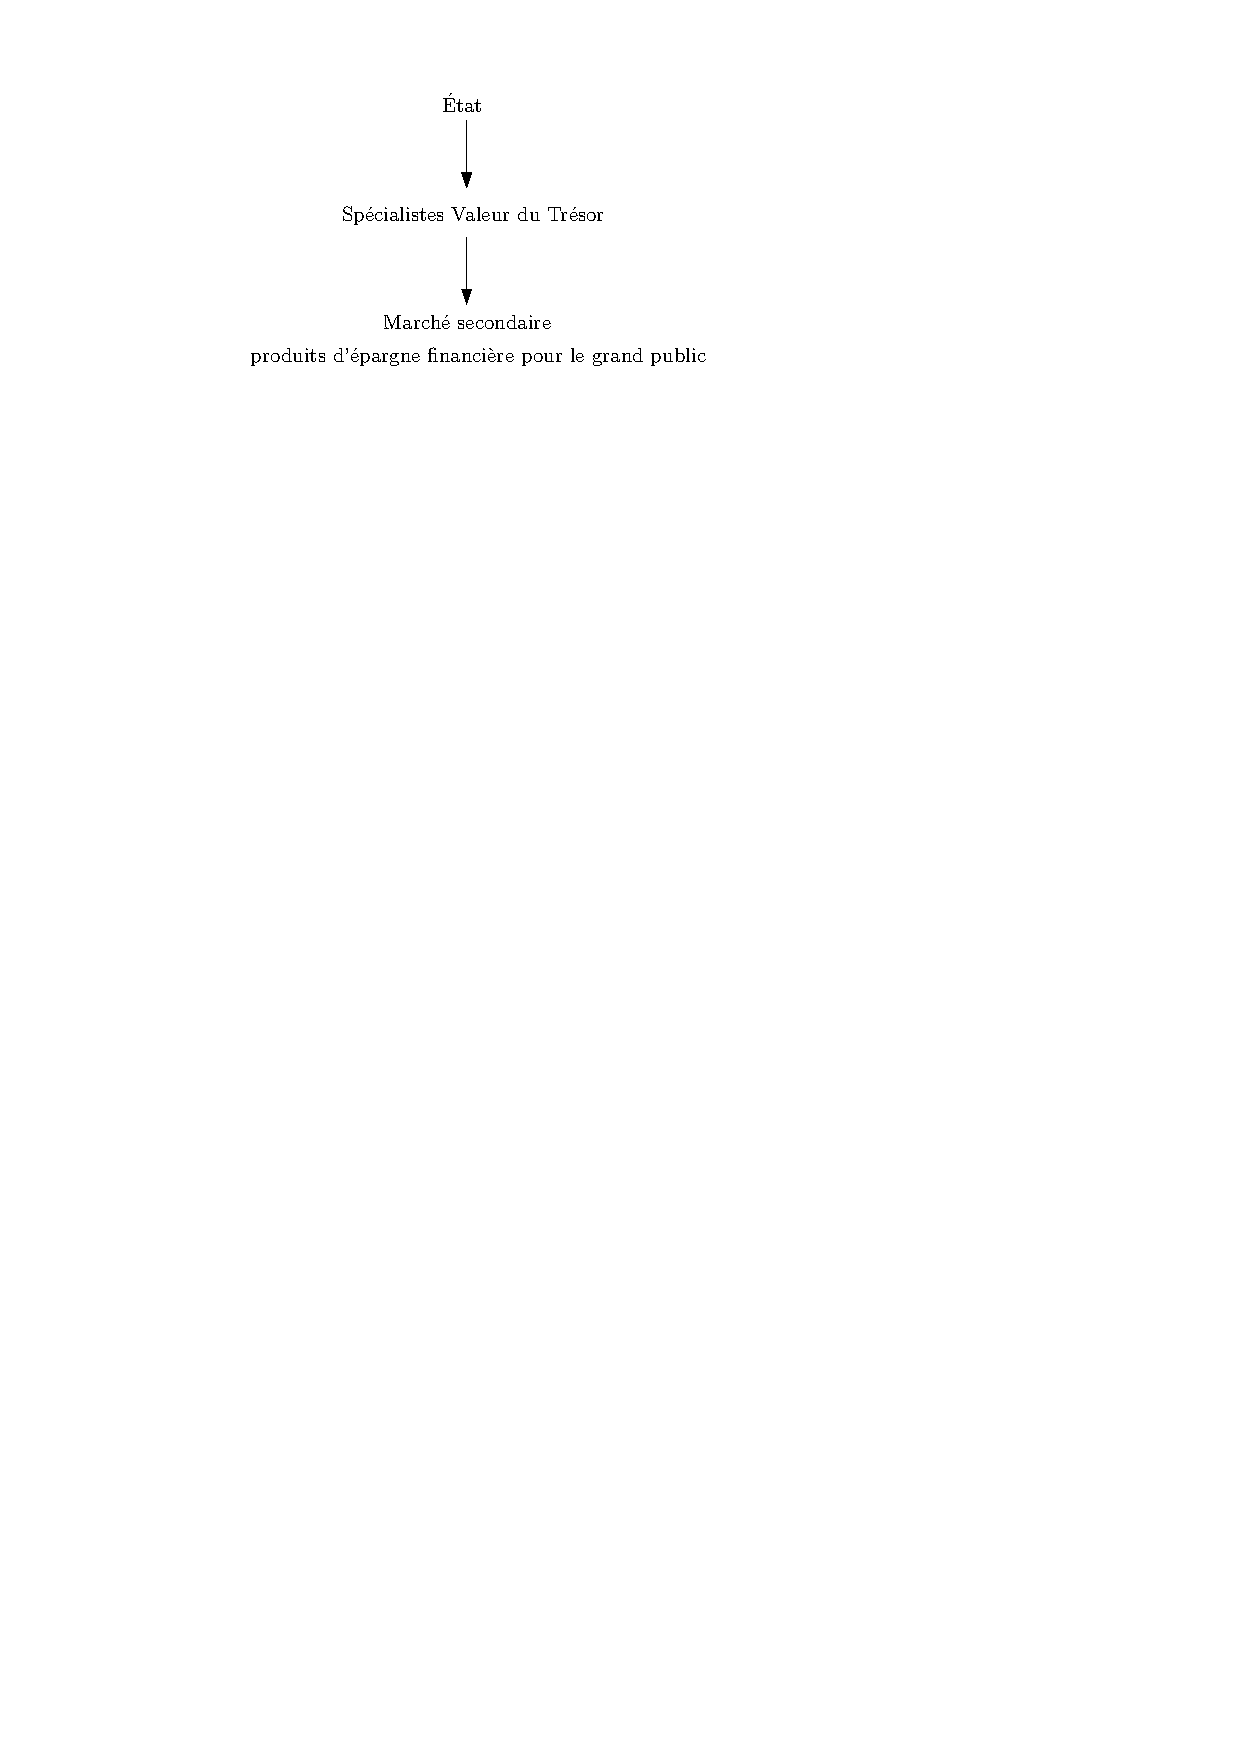
\includegraphics[width=0.8\textwidth]{dette.pdf}
                \caption{Schéma du rachat de la dette publique}
                \label{fig:dette}
        \end{figure}

Les dettes de l'État sont considérées comme un actif sûr, cela explique entre autres pourquoi malgré la valeur effarante de la dette publique les investisseurs continuent à prêter à l'État. Elles présentent plusieurs avantages:
\begin{itemize}
        \item Support de nombreux produits d'épargne à long terme comme les assurances vie
        \item Elles sont conservés par les investisseurs institutionnels
        \item Elles sont importantes pour les banques privées, ce sont des placements sans risque, éventuellement dans la monnaie nationale, et sont indispensables pour emprunter auprès de la Banque Centrale
\end{itemize}

\subsection{Les dettes publiques européennes}

\begin{definition}[Taux d'endettement]
       Il s'agit du rapport \[
               \frac{\text{Dette publique}}{\text{PIB}}
       .\] De par sa définition, l'évolution de ce ratio va dépendre, en plus des autres variables déjà identifiées, du taux de croissance de l'économie. 

\end{definition}

En 1992, lors du traité de Maastricht, il est fixé que ce rapport ne doit pas dépasser 60\%, et le déficit public doit être inférieur à 3\%. On parle de \emph{critère de Maastricht}, ou \emph{critère de convergence}. Ce seuil fut beaucoup critiqué car largement dépassé pour la plupart des pays européens, notamment la France et l'Allemagne qui disposent d'une économie robuste et réputée très solvable. En chiffres, le taux d'endettement français est proche de 100\%, cela représente un déficit de 2500 milliards d'euros. Il fut finalement  l'objet d'un assouplissement en Mars 2005 sous la pression de l'Allemagne et la France. \\
\begin{figure}[h!]
        \centering
        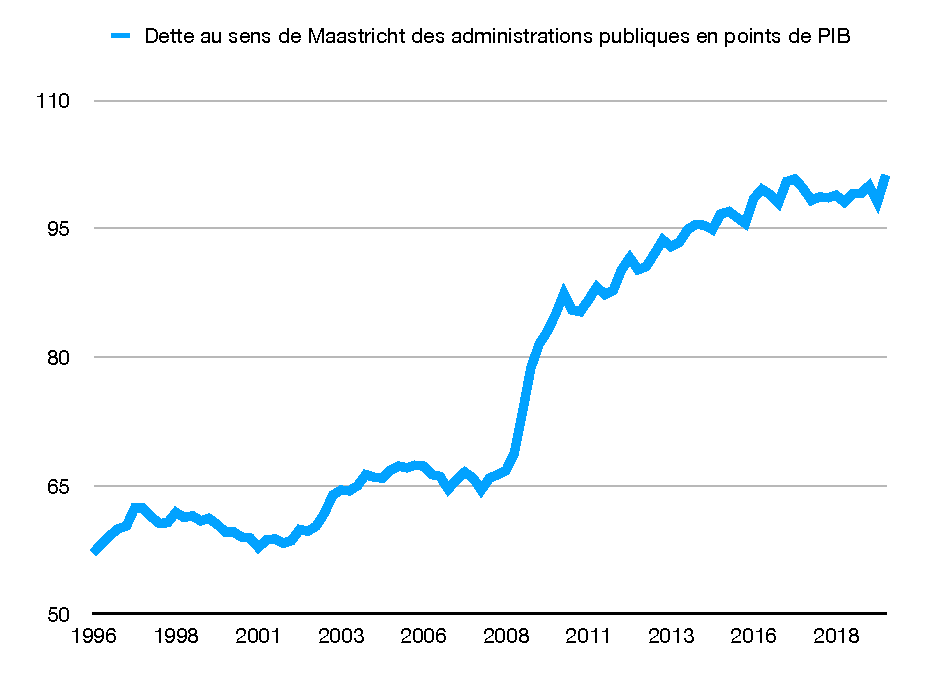
\includegraphics[width=0.8\textwidth]{dette_maa.pdf}
        \caption{Dette publique de l'État français au sens de Maastricht, source INSEE}
        \label{fig:dette_maa-pdf}
\end{figure}

\begin{definition}[Dette au sens de Maastricht]
       La dette au sens de Maastricht couvre l'ensemble des administrations publiques au sens des comptes nationaux. Sont ainsi pris en compte les passifs de l'État, des organismes divers d'administration centrale, des administrations publiques locales et des administrations de sécurité sociale. La dette au sens de Maastricht est une dette brute: on ne lui soustrait pas les actifs financiers que détiennent les administrations publiques. \\
       Le traité de Maastricht, entré en vigueur le 1er novembre 1993, a défini cinq critères de convergence que les États membres doivent respecter pour passer à la monnaie unique, l'euro. Les deux critères définis précédemment sont relatifs à la maîtrise des déficits publics.
\end{definition}


Une dette publique élevée n'est pas nécessairement signe d'une mauvaise économie, au contraire un pays aura intérêt à s'endetter lorsque son économie est en bonne santé et que les taux d'intérêt sont au plus bas, pour optimiser son développement. La réciproque n'est pas forcément vraie non plus, l'Espagne respectait le critère de Maastricht avant la crise de 2008 alors que son économie n'est pas la plus robuste d'Europe, le pays fut l'un des plus touché par la crise de l'euro de 2010. On observe une decorrelation générale entre la valeur de la dette publique et l'économie d'un pays, le cas de la Grèce semble aller à l'encontre de cette idée. \\

On peut cependant remarquer une corrélation entre l'apparition de crises économiques et l'augmentation de la dette publique des États touchés
\begin{itemize}
        \item Lors de la crise des \emph{subprime} et celle du \emph{Covid} le taux d'endettement de certains pays européens, et même des États Unis, a augmenté de 20 points
        \item Ce fut également le cas lors de la crise de l'euro en 2010, les pays les plus touchés furent la Grèce, puis l'Irlande, le Portugal et enfin l'Espagne
\end{itemize}
La crise des \emph{subprime} a eu des répercussions terribles en Europe, elle a induit la crise de l'euro de 2010, certains pays ne pouvaient plus se redresser.
Bien que les agences de notation jouent un rôle important dans ces situations de crise; ces dernières donnent une note qui définit un taux d'intérêt\footnote{Les taux fixés peuvent même être négatifs, ce qui induit un profit vis à vis de l'inflation et offre un placement sûr} auquel un État peut emprunter, en mai 2010, même avant leur intervention, la Grèce ne pouvait plus financer son rétablissement, elle fut suivie par une majorité des pays du sud de l'Europe. \\ 

Cette crise ne fut pas mondiale, bien que le résultat de la crise de 2008 qui elle l'était. A son origine on retrouve le fonctionnement particulier du système économique européen. Le traité de Lisbonne, signé en 2009, affirme l'indépendance de la BCE. Cette dernière ne peut prêter directement aux pays membres de l'Union Européenne, les États membres doivent respecter des règles strictes sur leur santé économique et financière et ce, sans se financer auprès de la BCE. \\

L'absence d'une véritable souveraineté européenne semble être le fond du problème, l'Europe n'est pas un pays, c'est un groupe très hétérogène d'États qui ne suivent pas les mêmes politiques budgétaires et n'ont pas de contrôle sur leur propre devise, ni même sur leur Banque Centrale qui est totalement indépendante.
Bien qu'assouplis, les critères de convergence stricts sont favorables à une politique de forte austérité plutôt qu'à la \emph{relance keynésienne}, et l'on peut se demander si cette politique n'a pas été à l'origine du déclin économique dont la Grèce peine toujours à se relever. Aujourd'hui les États européens n'abordent plus une crise économique de cette façon, en un sens s'endetter ne fait plus peur. L'INSEE recense une augmentation de la dette publique européenne de 58,4 milliards d'euros au premier semestre de 2020, suite à l'épidémie.

\subsection{Taux d'intérêts}

\textit{Les taux d'intérêt peuvent ils rester durablement très bas ?}

\bigskip

En Europe, c'est la BCE qui est en charge de la politique monétaire, elle est indépendante de tout État. Sa politique monétaire suit un cycle économique: lors d'une période de diminution de la croissance elle réduit les taux d'intérêts ce qui induit une hausse de la consommation et de l'inflation. Elle les remonte enfin lorsque l'inflation atteint un certain seuil pour éviter que les consommateurs ne perdent trop de pouvoir d'achat. \\

Ces taux sont aujourd'hui bas très bas, Japon + 20 ans avec un taux à 0\%, une inflation qui peine à augmenter, la comparaison zone Euro Japon a ses limites, crise démographique, taux d'endettement, etc.

Wicksel, taux intérêt naturel -> long terme s'accompagne d'une inflation stable, l'estimation de ce taux est basse

Causes structurelles
Excès d'épargne mondiale, liée à la hausse des inégalités et l'augmentation de l'espérance de vie
Demande d'investissement moindre

Certains désirent continuer cette politique jusqu'à obte,ir un taux à 2\%


Peuvent ils remonter?
Difficultés éventuelles des institutions financières
Risque de bulle économique
Nécessite pour les Banques Centrales de retrouver une marge de manoeuvre suffisante pour faire face à une nouvelle crise tout en composant avec l'existence d'une trappe à liquidité


Pourraient ils descendre plus bas?
Espèces pas disponibles, taux bas incitent crédit et investissent
Espèces disponibles, taux intérêts suffisamment bas, il est préférable d'épargner, rôle de plancher des taux d'intérêt

FMI suggère la création d'un système dual espèce/monnaie électronique 
\end{document}
